\newprob{1719220580}
{
    % active phys p283 q5
    就以下各情況,回答所有問題。
    \par{\par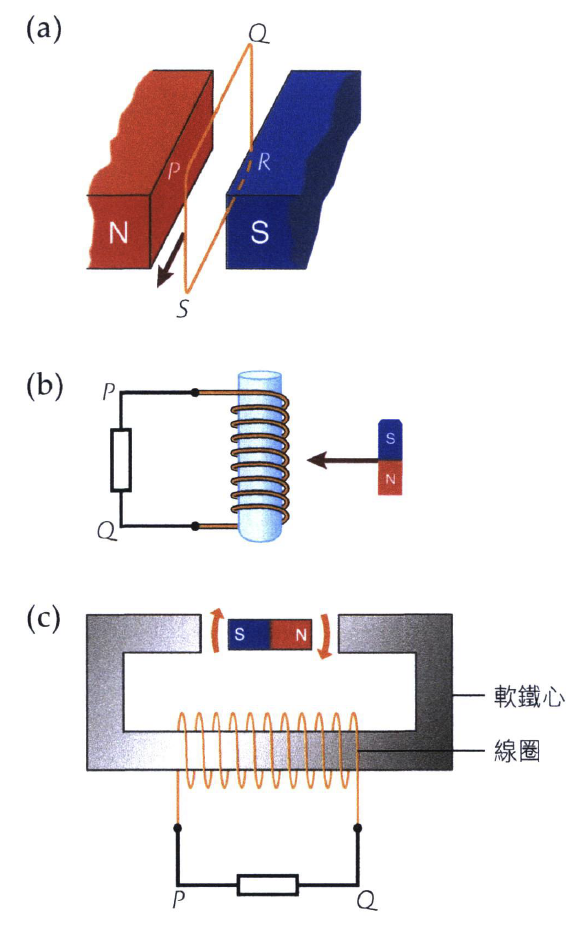
\includegraphics[width=.35\textwidth]{./img/ch5_induction_lq_2024-06-24-17-25-22.png}\par}
    \begin{subparts}
        \subpart 線圈所包圍的磁場有甚麽變化?
        \subpart 為抗衡這變化,線圈中的感生電流所產 生的磁場應指向哪一方?
        \subpart 試指出線圈中的感生電流方向。
    \end{subparts}
    \par \zzh{6}
}{\par{\par\centering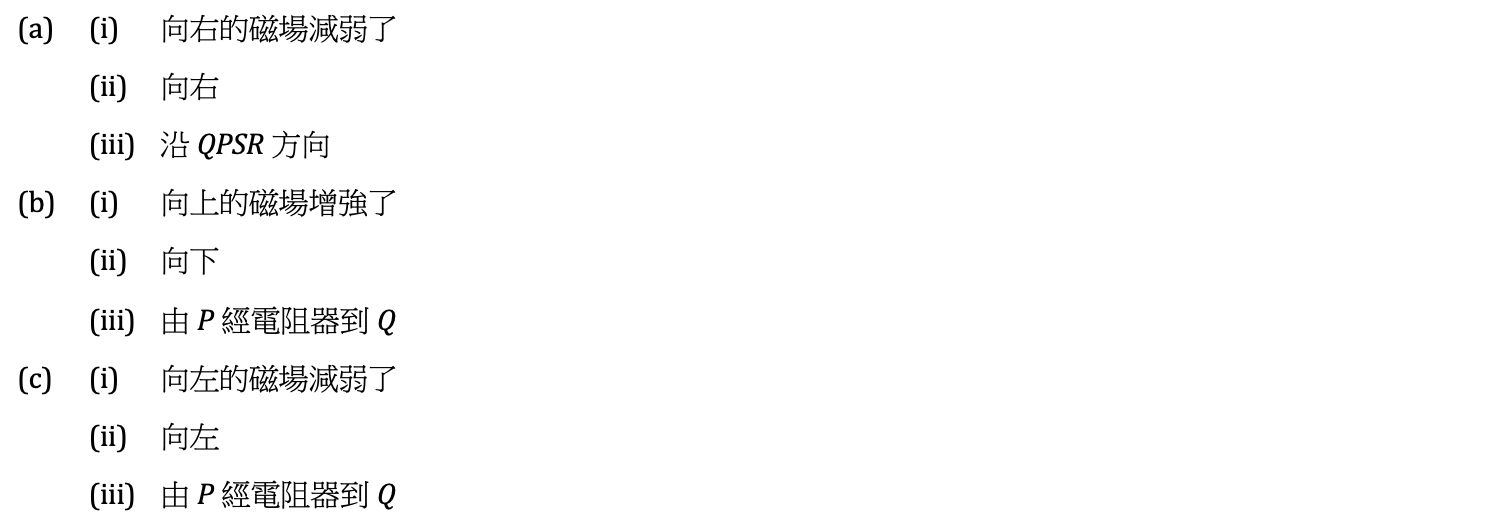
\includegraphics[width=\textwidth]{./img/ch5_induction_lq_2024-06-24-17-36-30.png}\par}}


\newprob{1719216705}
{
    % active phys p280 q1
    在一根固定的磁棒上,從靜止釋放一個金屬環。金屬環下墜時通 過磁棒,如圖。
    \par{\par\centering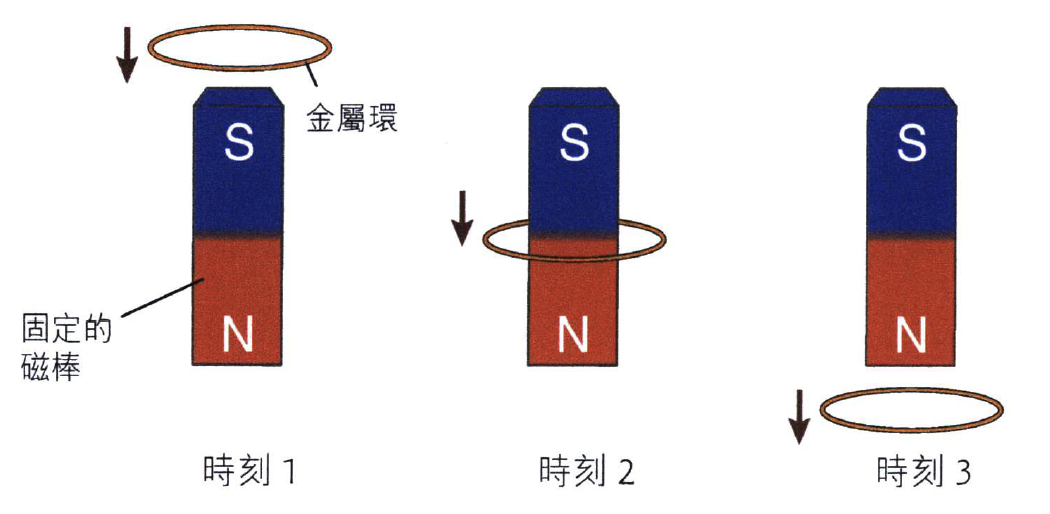
\includegraphics[width=.6\textwidth]{./img/ch5_induction_lq_2024-06-24-16-12-28.png}\par}
    從上方觀察,取順時針方向為正。
    \begin{parts}
        \part 指出在時刻1、2和3,金屬環上的感生電流方向,並扼要解 釋你的答案。(假設觀察者從上方望向金屬環。)\zzh{3}
        \part 線圖顯示感生電流I隨時間t的變化。
        \par{\par\centering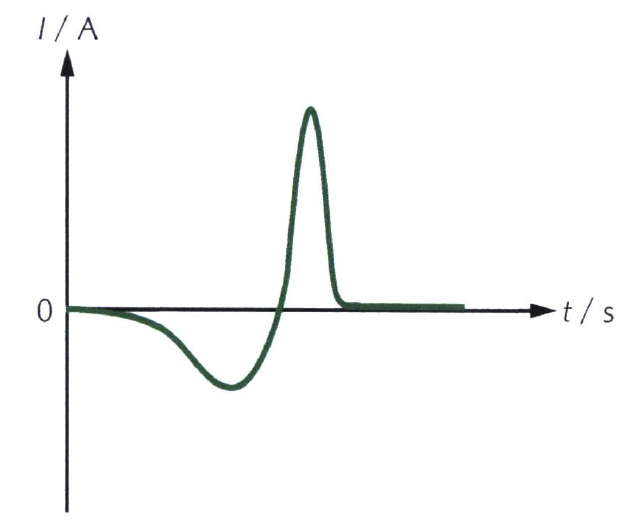
\includegraphics[width=.3\textwidth]{./img/ch5_induction_lq_2024-06-24-16-14-01.png}\par}
        試扼要解釋以下兩項。
        \begin{subparts}
            \subpart 為甚麼兩個峯正負相反?\zzh{1}
            \subpart 為甚麼第二個峯比第一個高? \zzh{1}
        \end{subparts}
        \part 金屬環下墜時的加速度不變嗎?試扼要解釋。\zzh{2}
    \end{parts}
    \dlines{1}\clearpage
}{
    % \src{Active physics p280 q1}
    \par{\par\centering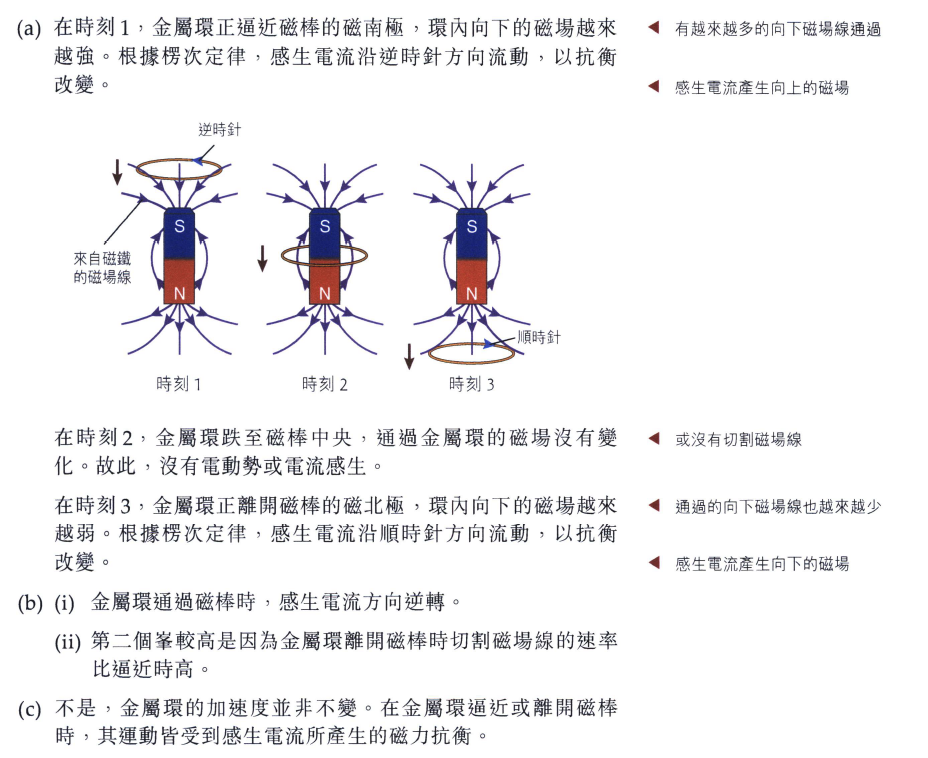
\includegraphics[width=\textwidth]{./img/ch5_induction_lq_2024-06-24-16-15-31.png}\par}
}


\newprob{1719221206}
{
    % active phys p283 q6 & 7
    一根首尾以導線相連的金屬棒通過一個勻強磁 場,如圖。
    \par{\par\centering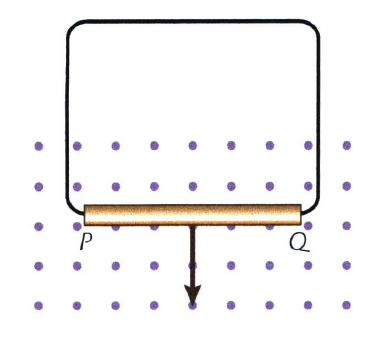
\includegraphics[width=.3\textwidth]{./img/ch5_induction_lq_2024-06-24-17-27-13.png}\par}
    \begin{parts}
        \part 為抗衡金屬棒向下的運動,所產生的磁力沿 哪一個方向作用在其上?\zzh{1}
        \part 若要產生這個磁力,感生電流應沿哪一個方 向流動?\zzh{1}
        \part 試利用弗林明右手定則,找出感生電流的方 向。答案與(b)部相符嗎?\zzh{1}
        \part 現把連接金屬棒兩端的導線移去。
        \begin{subparts}
            \subpart 金屬棒上有任何感生電流嗎?為甚麼?\zzh{2}
            \subpart 電子累積在金屬棒哪一端?試扼要解釋。\zzh{2}
            \subpart 由此,指出金屬棒哪一端的電勢較高。\zzh{1}
        \end{subparts}
    \end{parts}
    \dlines{1}\clearpage
}{\par{\par\centering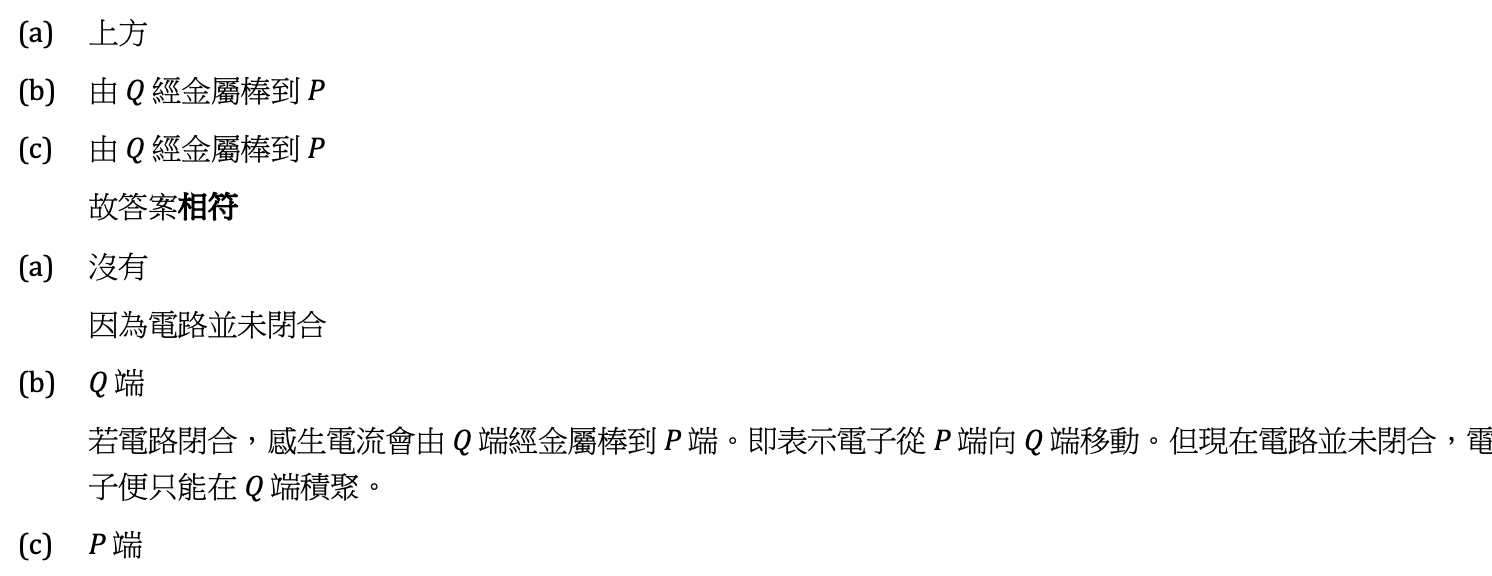
\includegraphics[width=\textwidth]{./img/ch5_induction_lq_2024-06-24-17-36-49.png}\par}}

\newprob{1719221432}
{
    % active phys p283 q10
    線圈P和Q繞在一根軟鐵棒上,如圖。
    \par{\par\centering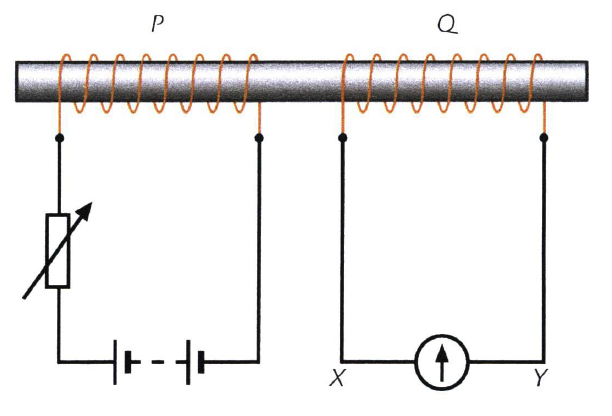
\includegraphics[width=.35\textwidth]{./img/ch5_induction_lq_2024-06-24-17-30-54.png}\par}
    變阻器的電阻減少至原來的一半,期間,電流在 線圈Q上感生。
    \begin{parts}
        \part 試指出感生電流的方向。\zzh{1}
        \part 舉出三個增加指針偏轉程度的方法。\zzh{3}
    \end{parts}
}{\par{\par\centering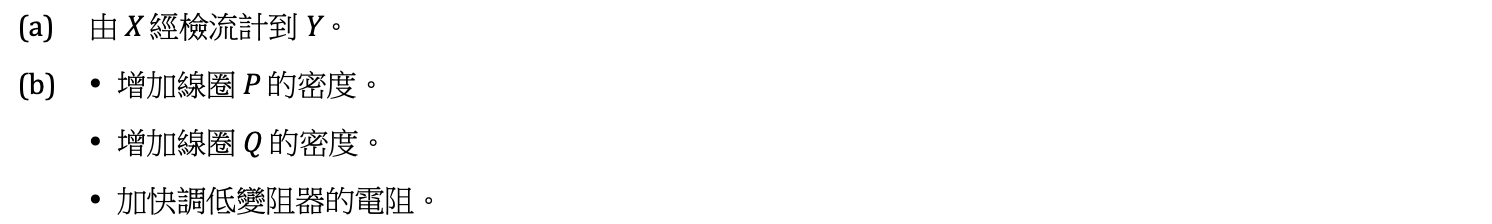
\includegraphics[width=\textwidth]{./img/ch5_induction_lq_2024-06-24-17-37-25.png}\par}}

\newprob{1719221292}
{
    % active phys p283 q12
    一個鋁環放在一個電磁鐵上。
    \par{\par\centering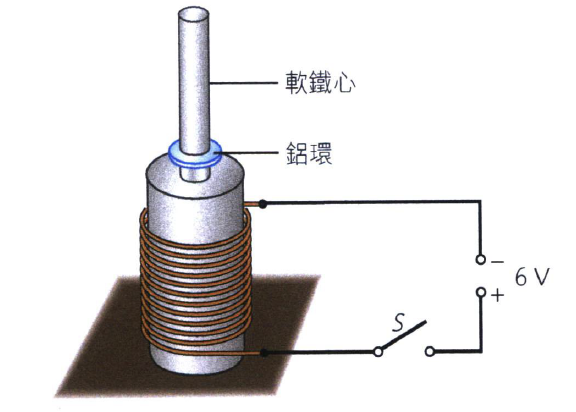
\includegraphics[width=.3\textwidth]{./img/ch5_induction_lq_2024-06-24-17-32-08.png}\par}
    在開關閉合的瞬間,鋁環躍起。
    \begin{parts}
        \part 鋁環其後會掉下還是浮在半空?試扼要解 釋。\zzh{3}
        \part 在以下各情況中,鋁環躍起的最大高度有甚 麼變化?\zzh{3}
        \begin{subparts}
            \subpart 螺線管多繞數匝
            \subpart 把軟鐵心換成紙筒
            \subpart 鋁環破開一道窄縫
        \end{subparts}
    \end{parts}
}{\par{\par\centering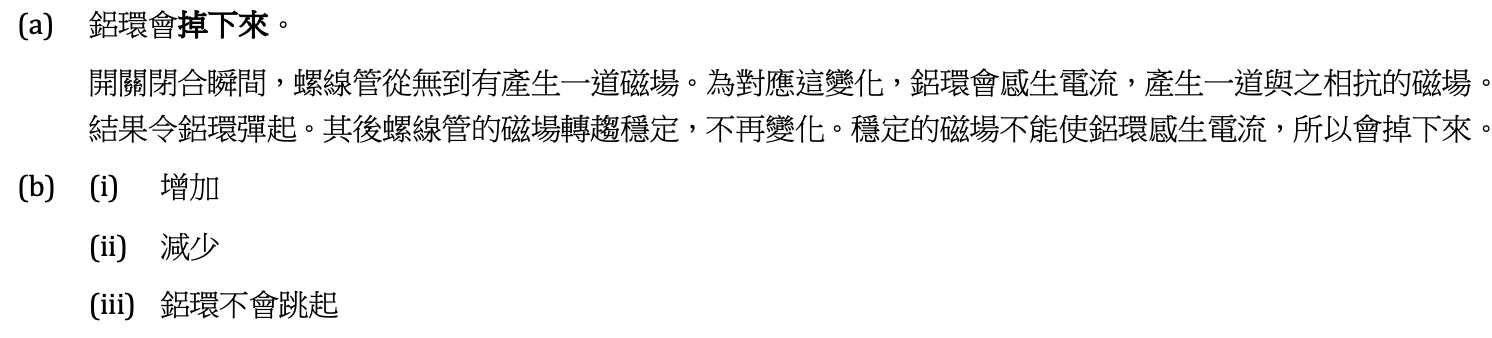
\includegraphics[width=\textwidth]{./img/ch5_induction_lq_2024-06-24-17-38-04.png}\par}}

\newprob{1719220094}
{
    % active phys p311 p6
    現有一個方形勻強磁場,由一個電阻為  \qty{20}{\ohm} 的 方形線圈包圍着,如圖。若磁場正以  \qty{0.2}{T.s^{-1}} 的 速率增加,求線圈上的感生電流。\zzh{2}
    \par{\par\centering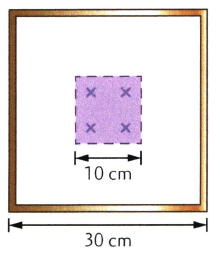
\includegraphics[width=.25\textwidth]{./img/ch5_induction_lq_2024-06-24-17-09-02.png}\par}
}{\par{\par\centering
\includegraphics[width=\textwidth]{./img/ch5_induction_lq_2024-06-24-17-39-15.png}\par}}

\newprob{1719220150}
{
    % active phys p311 q7
    小珍製作了一個簡單發電機,所用的磁鐵能產生 量值為0.5 T的勻強磁場。線圈共有50匝,以 2 Hz 的頻率在磁鐵之間旋轉,並連接至一個  \om{10} 電阻器。現在,小珍正估計發電機的輸出功率。
    \par{\par\centering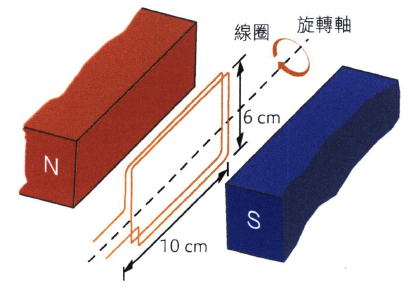
\includegraphics[width=.3\textwidth]{./img/ch5_induction_lq_2024-06-24-17-11-57.png}\par}

    \begin{parts}
        \part 當線圈旋轉了 \dg{90},磁通量的變化為多少?\zzh{2}
        \part 由此,求線圈上的平均感生電動勢。\zzh{2}
        \part 由此,估計發電機的輸出功率。\zzh{2}
    \end{parts}
}{\par{\par\centering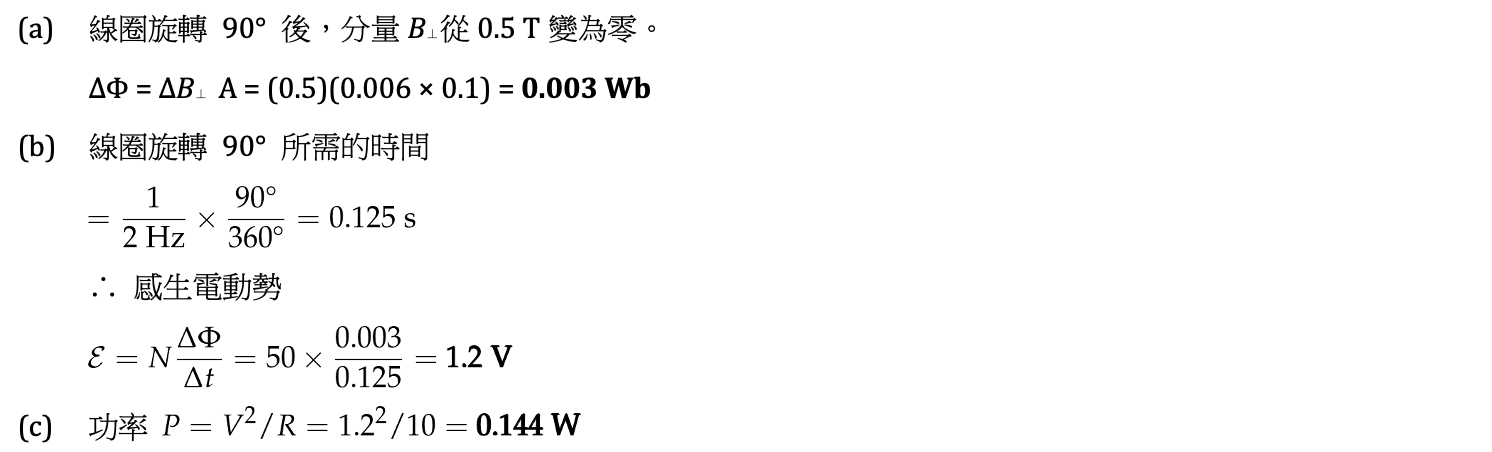
\includegraphics[width=\textwidth]{./img/ch5_induction_lq_2024-06-24-17-39-28.png}\par}}

\newprob{1719220375}
{
    % active phys p311 q10
    一個銅線框質量為4 g,電阻為\om{20},在某高度 上從靜止釋放。銅線框其後以勻速通過一個量值 為1 T的勻強磁場,如圖。空氣阻力的影響可略 去不計。已知重力加速度為 \acc{9.81}。
    \par{\par\centering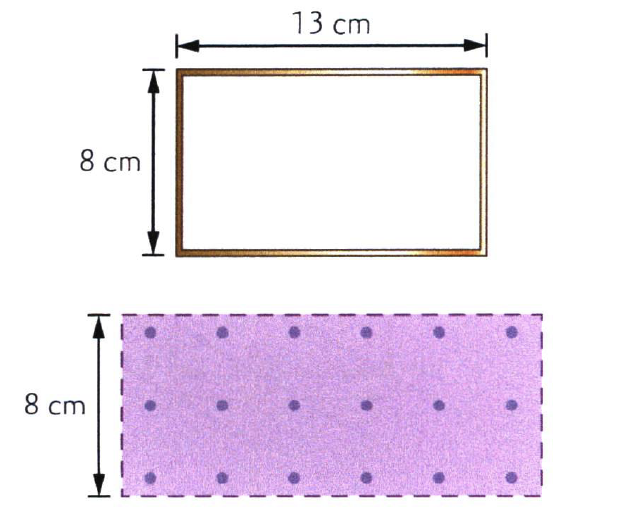
\includegraphics[width=.3\textwidth]{./img/ch5_induction_lq_2024-06-24-17-14-06.png}\par}

    \begin{parts}
        \part 求金屬框中的感生電流。\zzh{2}
        \part 通過該區域時,散失的總能量為多少?\zzh{2}
    \end{parts}
}{\par{\par\centering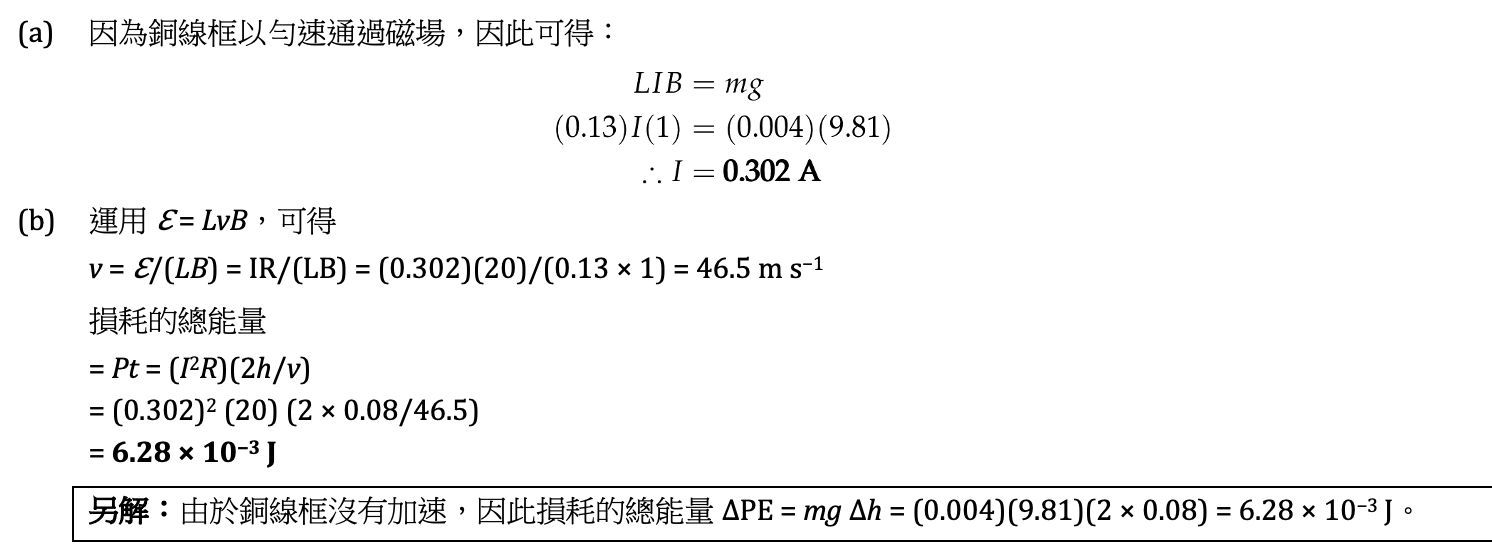
\includegraphics[width=\textwidth]{./img/ch5_induction_lq_2024-06-24-17-39-43.png}\par}}

\newprob{1719220468}
{
    % active phys p311 q11
    一根電阻可忽略的導電棒放在一對平行的平滑路 軌上,如圖。導電棒與路軌成某角度,正以 2 m s-'的速率推向右方。整個裝置處於一個匀 強磁場內,量值為0.4T,方向指入紙面。
    \par{\par\centering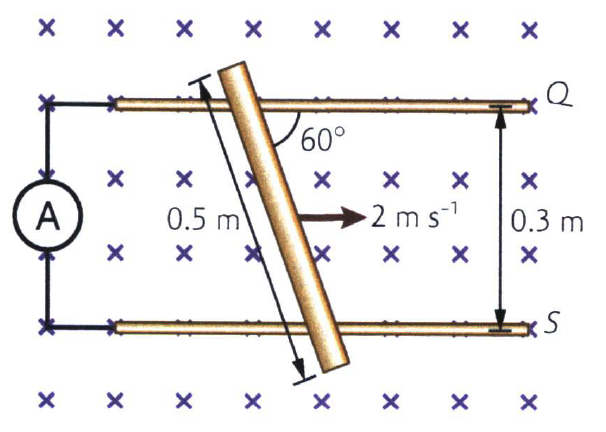
\includegraphics[width=.35\textwidth]{./img/ch5_induction_lq_2024-06-24-17-15-08.png}\par}
    \begin{parts}
        \part 求QS 兩點的感生電動勢。\zzh{2}
        \part 以下的改變對感生電動勢有甚麼影響?\zzh{3}
        \begin{subparts}
            \subpart 進一步減小導電棒與路軌之間的夾角
            \subpart 增加路軌之間的距離
            \subpart 增加路軌的電阻
        \end{subparts}
    \end{parts}
}{\par{\par\centering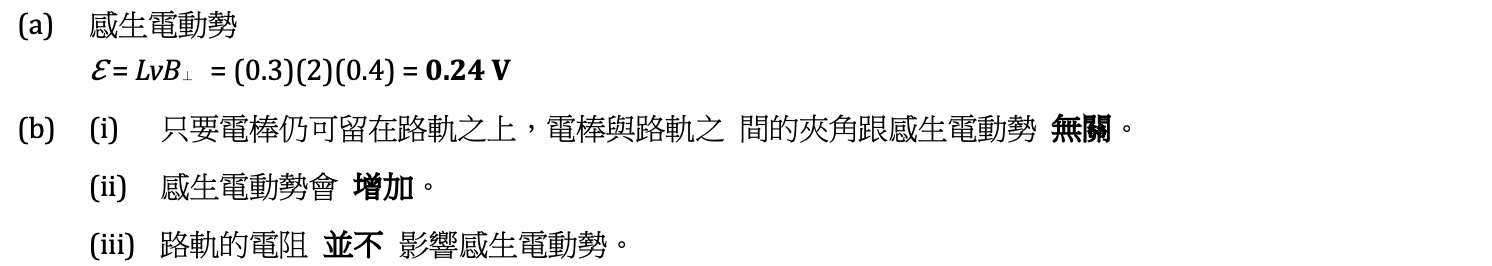
\includegraphics[width=\textwidth]{./img/ch5_induction_lq_2024-06-24-17-39-56.png}\par}}

